\documentclass[class=article, crop=false]{standalone}
\usepackage{tikz}
\usepackage{subcaption}
\usetikzlibrary{calc}
\usetikzlibrary {shapes.geometric}

\begin{document}
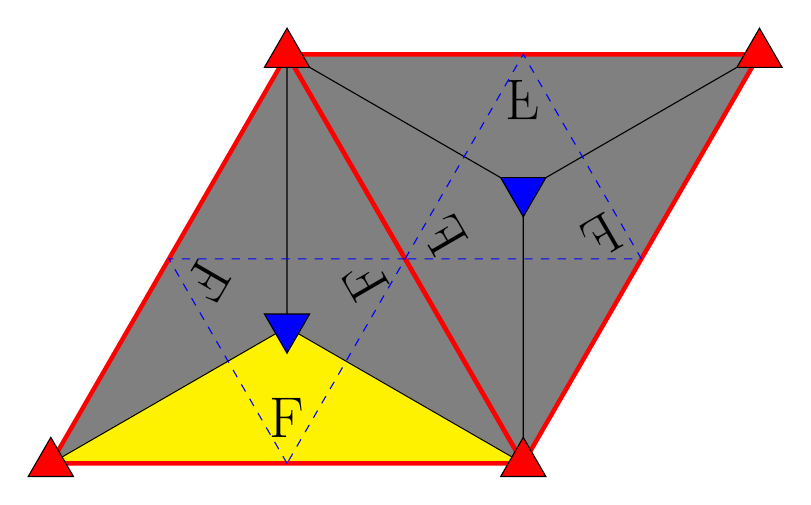
\begin{tikzpicture}
            % Define the lengths of the sides and the angle
            \def\a{3}  % length of side a
            \def\b{3}  % length of side b
            \def\angle{60}  % angle between sides a and b
            \def\s{F} % Label in center of cells

            \def\x{0.5} % Boundary 
            \def\y{0.5} % Boundary
        
            % Calculate the coordinates of the points
            \coordinate (C00) at (0, 0);
            \coordinate (C10) at (\a, 0);
            \coordinate (C11) at ({\a + \b*cos(\angle)}, {\b * sin(\angle)});
            \coordinate (C01) at ({\b * cos(\angle)}, {\b * sin(\angle)});
            \coordinate (C02) at ({2*\b*cos(\angle)}, {2*\b * sin(\angle)});
            \coordinate (C12) at ({\a +2*\b * cos(\angle)}, {2*\b * sin(\angle)});
            \coordinate (C22) at ({2*\a + 2*\b * cos(\angle)}, {2*\b * sin(\angle)});
            \coordinate (C21) at ({2*\a + \b*cos(\angle)}, {\b * sin(\angle)});
            \coordinate (C20) at ({2*\a}, 0);

            \coordinate (A1) at ($(C00)!0.6666!(C11)$);
            \coordinate (A2) at ($(C11)!0.3333!(C22)$);
        
            % Draw the oblique unit cell
            \draw[fill=gray,gray] (C00) -- (C20) -- (C22) -- (C02) -- cycle;
            \draw[fill=yellow,yellow] (C00) -- (A1) -- (C20) -- cycle;
            
            
            
            % Draw chiral center
            \node at ($(C00)!0.5!(C20)!0.3333!(A1)$) {\huge \s};
            \node[rotate=240] at ($(C00)!0.5!(C02)!0.3333!(A1)$) {\huge \s};
            \node[rotate=120] at ($(C20)!0.5!(C02)!0.3333!(A1)$) {\huge \s};
            \node[rotate=300] at ($(C20)!0.5!(C02)!0.3333!(A2)$) {\reflectbox{\huge \s}};
            \node[rotate=30] at ($(C20)!0.5!(C22)!0.3333!(A2)$) {\reflectbox{\huge \s}};
            \node[rotate=180] at ($(C02)!0.5!(C22)!0.3333!(A2)$) {\reflectbox{\huge \s}};

            % Draw mirrow lines
            \draw[ultra thick,red] (C00) -- (C02) -- (C20) -- cycle;
            \draw[ultra thick,red] (C02) -- (C22) -- (C20) -- cycle;
            \draw[thin] (C00) -- (A1) -- (C02) -- (A2) -- (C22);
            \draw[thin] (A1) -- (C20) -- (A2);
            \draw[dashed,blue] (C10) -- (C01) -- (C11) -- cycle;
            \draw[dashed,blue] (C11) -- (C12) -- (C21) -- cycle;
            

            % Draw node rotations symbols
            \draw (C00)  node[regular polygon, regular polygon sides=3, draw, fill=red, minimum size=0.5cm] {};
            \draw (C02)  node[regular polygon, regular polygon sides=3, draw, fill=red, minimum size=0.5cm] {};
            \draw (C22)  node[regular polygon, regular polygon sides=3, draw, fill=red, minimum size=0.5cm] {};
            \draw (C20)  node[regular polygon, regular polygon sides=3, draw, fill=red, minimum size=0.5cm] {};

            \draw (A1)  node[rotate = 180,regular polygon, regular polygon sides=3, draw, fill=blue, minimum size=0.5cm] {};
            \draw (A2)  node[rotate=180, regular polygon, regular polygon sides=3, draw, fill=blue, minimum size=0.5cm] {};

        \end{tikzpicture}
\end{document}